%%%%%%%%%%%%%%%%%%%%%%%%%%%%%%%%%%%%%%%%%
% Beamer Presentation
% LaTeX Template
% Version 1.0 (10/11/12)
%
% This template has been downloaded from:
% http://www.LaTeXTemplates.com
%
% License:
% CC BY-NC-SA 3.0 (http://creativecommons.org/licenses/by-nc-sa/3.0/)
%
%%%%%%%%%%%%%%%%%%%%%%%%%%%%%%%%%%%%%%%%%

%----------------------------------------------------------------------------------------
%	PACKAGES AND THEMES
%----------------------------------------------------------------------------------------

\documentclass{beamer}

\mode<presentation> {

% The Beamer class comes with a number of default slide themes
% which change the colors and layouts of slides. Below this is a list
% of all the themes, uncomment each in turn to see what they look like.

%\usetheme{default}
%\usetheme{AnnArbor}
%\usetheme{Antibes}
%\usetheme{Bergen}
%\usetheme{Berkeley}
%\usetheme{Berlin}
%\usetheme{Boadilla}
%\usetheme{CambridgeUS}
%\usetheme{Copenhagen}
%\usetheme{Darmstadt}
%\usetheme{Dresden}
%\usetheme{Frankfurt}
%\usetheme{Goettingen}
%\usetheme{Hannover}
%\usetheme{Ilmenau}
%\usetheme{JuanLesPins}
%\usetheme{Luebeck}
\usetheme{Madrid}
%\usetheme{Malmoe}
%\usetheme{Marburg}
%\usetheme{Montpellier}
%\usetheme{PaloAlto}
%\usetheme{Pittsburgh}
%\usetheme{Rochester}
%\usetheme{Singapore}
%\usetheme{Szeged}
%\usetheme{Warsaw}

% As well as themes, the Beamer class has a number of color themes
% for any slide theme. Uncomment each of these in turn to see how it
% changes the colors of your current slide theme.

%\usecolortheme{albatross}
%\usecolortheme{beaver}
%\usecolortheme{beetle}
%\usecolortheme{crane}
%\usecolortheme{dolphin}
%\usecolortheme{dove}
%\usecolortheme{fly}
%\usecolortheme{lily}
%\usecolortheme{orchid}
%\usecolortheme{rose}
%\usecolortheme{seagull}
%\usecolortheme{seahorse}
%\usecolortheme{whale}
%\usecolortheme{wolverine}

%\setbeamertemplate{footline} % To remove the footer line in all slides uncomment this line
%\setbeamertemplate{footline}[page number] % To replace the footer line in all slides with a simple slide count uncomment this line

%\setbeamertemplate{navigation symbols}{} % To remove the navigation symbols from the bottom of all slides uncomment this line
}
\usepackage[brazil]{babel} % pacote portugues brasileiro
\usepackage[utf8]{inputenc} % pacote para acentuacao direta
\usepackage{graphicx} % Allows including images
\usepackage{booktabs} % Allows the use of \toprule, \midrule and \bottomrule in tables

%----------------------------------------------------------------------------------------
%	TITLE PAGE
%----------------------------------------------------------------------------------------

\title{Proposta de um Modelo para Representar Cenários de Acidentes Usando Conceitos de Normas, Sanções e Violações} % The short title appears at the bottom of every slide, the full title is only on the title page

\author{Jonathan M. Samara \\ Orientador Prof. Dr. Cesar A. Tacla} % Your name
\institute[UTFPR] % Your institution as it will appear on the bottom of every slide, may be shorthand to save space
{
Universidade Tecnológica Federal do Paraná \\ % Your institution for the title page
\medskip
}
\date{\today} % Date, can be changed to a custom date

\begin{document}

\begin{frame}
\titlepage % Print the title page as the first slide
\end{frame}

\begin{frame}
\frametitle{Introdução} % Table of contents slide, comment this block out to remove it
	\begin{itemize}
			\item Muitas pessoas são submetidas a atividades que apresentam algum risco. 
			\item Exemplos de serviços assim; elétrica, petroquímica, telecomunicações, transportes. 
			\item Existe uma série de possíveis causas em um acidente. 
			\item A computação pode contribuir com esse tipo de problema. 
			\item Criar representações para tratar esse problema. 			
	\end{itemize}
\end{frame}

\begin{frame}
\frametitle{Introdução - Motivação} % Table of contents slide, comment this block out to remove it
	\begin{itemize}
			\item Uma maneira de representar cenários assim está relacionado com sistemas multiagentes normativos. 
			\item Dentro deste tipo de atenge é possível observar os conceitos de; norma, violação e sanção.
			\item Portanto, entender como usar agentes normativos para criar representações específicas a problemas envolvendo trabalho, acidente e risco é uma motivação para esse estudo. 
			\item Realizar a análise dos raciocínios que podem ser construído é outra motivação. 			
	\end{itemize}
\end{frame}

\begin{frame}
\frametitle{Introdução - Relevância} % Table of contents slide, comment this block out to remove it
	\begin{itemize}
			\item Contribuição para três campos; Representação Computacional, Sistemas Multiagentes e Segurança.
			\item Representação Computacional e Sistemas Multiagentes.
			\begin{itemize}
				\item Existem modelos para representar Sistemas Multiagentes, porém não apresentam características específicas (conceitos, predicados, regras) para tratar cenários de acidentes. 
				\item Existem modelos para representar SMA Normativos, mas apresentam aspectos altamente genéricos, não tendo características específicas (conceitos, predicados e regras) para tratar cenários de acidentes e riscos.
				\item Existem modelos para representar cenários de acidentes (am ambiente de trabalho) usando \textit{SMA}, contudo são complexos. Além disso, esses modelos não focam no erro dos agentes bem como as consequências dos mesmos sobre os demais colegas.  
			\end{itemize}			 
	\end{itemize}
\end{frame}

\begin{frame}
\frametitle{Introdução - Relevância} % Table of contents slide, comment this block out to remove it
	\begin{itemize}
			\item Segurança
			\begin{itemize}
				\item O interesse da pesquisa é computacional. 
				\item O modelo aqui proposto trata de conceitos relacionados a riscos e situações inesperadas.
				\item Portanto, apesar do interesse ser principalmente computacional, há um diálogo com o campo da Segurança. 
			\end{itemize}			 
	\end{itemize}
\end{frame}

\begin{frame}
\frametitle{Introdução - Objetivo Geral} % Table of contents slide, comment this block out to remove it
	\begin{itemize}
		\item Conceber uma representação que tenha maior expressividade (quando comparado com os demais modelos) ao representar o seguinte cenário; "Agentes trabalham de forma colaborativa para atingir um dado objetivo geral. Esses agentes podem cometer erros submetendo a si mesmos bem como a outros a acidentes ocasionando grandes danos a integridade física do(s) acidentado(s). Não apenas isso, mas essa representação deverá ser capaz de considerar as relações existentes entre as entidades (agentes, artefatos tais como ferramentas), condições ambientais com as violações, sanções e acidentes. Questões envolvendo caráter possibilístico dos acidentes frente a ação dos agentes também deverão ser verificadas nessa representação."  
	\end{itemize}
\end{frame}

\begin{frame}
\frametitle{Introdução - Objetivos Específicos}
	\begin{enumerate}
		\item Representar um SMA. 
		\item Representar normas, violações e sanções sendo que as violações são erros cometidos pelos agentes e as sanções estão relacionadas com os acidentes e suas respectivas consequências.
		\item Representar situações onde um agente é submetido a um evento ruim (integridade física do agente é negativamente afetada de alguma maneira) mesmo que ele não tenha cometido erro algum. 
		\item Representar como se dá as relações entre as entidades, condições ambientes e conjunto coma s violações e sanções. 
		\item Representar as possibilidades da ocorrência de um evento atrelado a um dado risco. 
	\end{enumerate}
\end{frame}


\begin{frame}
\frametitle{Fundamentação Teórica - Agentes}
	\begin{itemize}
		\item Um agente é um sistema computacional que está situado em um dado ambiente e que apresenta comportamento autônomo com a finalidade de atingir um dado objetivo que a ele é designado. 
		\item Um agente pode ser estruturado em termos \textit{goal-governed} e \textit{goal-oriented}.
		\item Os agentes \textit{goal-governed} têm capacidades cognitivas e podem representar os seus respectivos objetivos. 
		\item Os agentes \textit{goal-oriented} são programados para alcançar um dado objetivo. 
		\item Artefatos não se enquadram nessas duas características. Essas entidades são exploradas pelo agente para que eles possam alcançar um dado objetivo. 
	\end{itemize}
\end{frame}

\begin{frame}
\frametitle{Fundamentação Teórica - SMA}
	\begin{itemize}
		\item Um sistema multiagente é constituído por agentes autônomos que interagem visando um propósito em comum tendo como consequência um comportamento global. 
		\item Uma organização com essas características, portanto, apresenta em comum; cultura, memória, história, distribuição de atividades e capacidade de distinguir um agente em específico. 
		\item Uma organização de sistema multiagente deve conter relações sociais no que tange a agentes, institutos específicos e grupos sociais. 
		\item Por ser uma organização, uma \textit{SMA} apresenta; Divisão de tipos de atividades, integração, composição, estabilidade/flexibilidade, coordenação, recursividade, representação multinível e causalidade, potenciais e diferenciais, regras e gramáticas.
	\end{itemize}
\end{frame}

\begin{frame}
	\frametitle{Fundamentação Teórica - Normas}
	\begin{figure}[H]
	  \centering
	  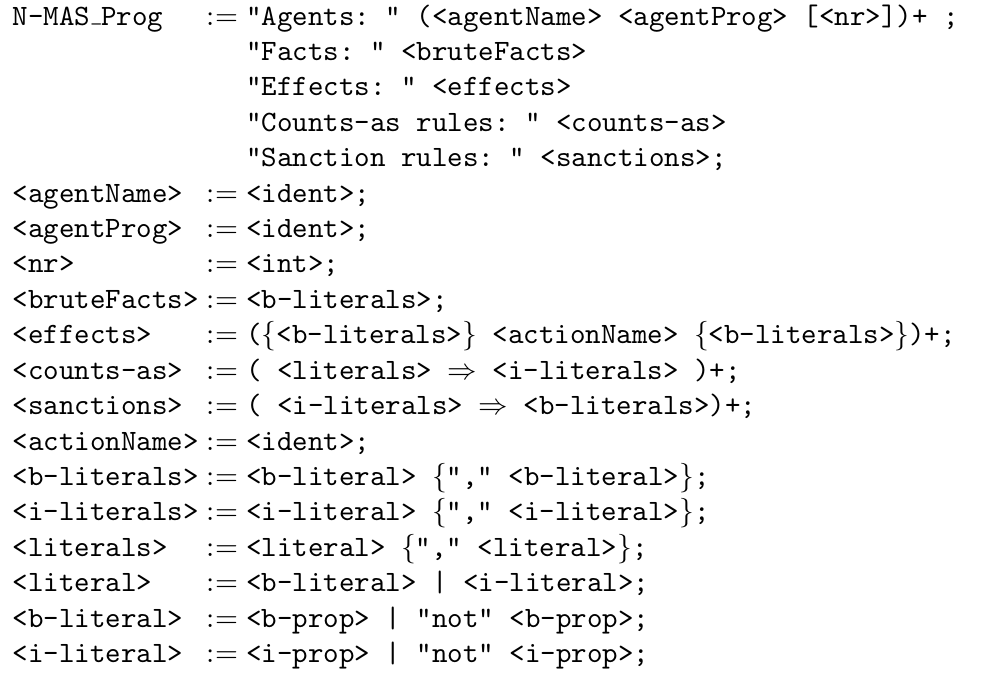
\includegraphics[width=0.5\linewidth]{figure/masprogram.png} 
	  \caption{Linguagem para descrever um programa de multiagentes normativos com a possibilidade de violações e sanções na notação EBNF segundo o texto \cite{dastaniframework}. Nesta notação, $<ident>$ é usado para denotar uma \textit{string} e $<int>$ inteiros. Os termos $<b-prop>$ e $<i-prop>$ são usados para designar dois tipos de conjuntos de proposições que são disjuntos entre si}
	  \label{descreveprograma}
	\end{figure}
\end{frame}


\begin{frame}
	\frametitle{Fundamentação Teórica - Riscos}
	\begin{itemize}
		\item BATU - \textit{Boundary Activities Tolerated during Use} (Atividades Limites Toleradas Durante o Uso). Muitas vezes a equipe adota atividades paliativas a fim de otimizar os processos de produção. Isso envolve assumir níveis de tolerância no que diz respeito ao desempenho e a segurança. 
		\item BCTU - \textit{Boundary Conditions Tolerated by Use} (Condições Limites Toleradas Durante o Uso). O termo condição faz referência a uma situação, um estado, circunstâncias externas às quais pessoas ou até mesmo entidades são afetados no que diz respeito a uma certa decisão atrelada a circunstâncias ambientais, materiais, humanas, de produtos e entre outras.
	\end{itemize}
\end{frame}

\begin{frame}
	\frametitle{Metodologia - Levantamento de Requisitos}
	\begin{itemize}
		\item Os requisitos são derivados de uma análise dos Objetivos Específicos desse estudo.
		\item Apresentam as seguintes características; 
		\begin{itemize}
			\item São estáticos (uma vez formulado o problema, não mudam com o decorrer do desenvolvimento da representação);
			\item São articulados em um vocabulário compreensível para o autor desta dissertação. 			
		\end{itemize}
	\end{itemize}
\end{frame}

\begin{frame}
	\frametitle{Metodologia - Conceitualização}
	\begin{itemize}
		\item Investigação de modelos que podem ser aplicados a essa situação.
		\item Verificação dos conceitos em interesse dentro desses modelos. 
		\item O autor isolou os conceitos e suas relações nesses modelos. 
		\item Os conceitos ão adaptados ao cenário que se deseja representar.
		\item A estrutura resultante é escrita no seguinte formalismo; Teoria de Conjuntos para representar os conceitos e lógica de predicados para representar as relações. 
		\item UML também é usado para essa mesmo propósito. 
		\item Uma vez feito isso, o autor elabora regras para determinar a transição as transições de estado.
	\end{itemize} 
\end{frame}

\begin{frame}
	\frametitle{Metodologia - Análise do Estudo de Caso}
	\begin{itemize}
		\item Manutenção em Linha Viva. 
		\item Estudo de manuais técnicos. 
		\item Entrevista com o Engenheiro de Manutenção de Linha Viva. 
		\item Acompanhamento de um procedimento de Manutenção. 
		\item É feito um Modelo Baseado em Cenários que consiste na descrição da atividade em linguagem natural. Esse modelo foi verificado por profissionais da área. 
		\item Desse houve o processo de especificação nos conjuntos e predicados definidos anteriormente. 
	\end{itemize} 
\end{frame}

\begin{frame}
	\frametitle{Metodologia - Validação}
	\begin{itemize}
		\item Uma vez com a manutenção especificada, o autor gera raciocínios para traduzir diferentes cenários de trabalho (com o propósito de provar a hipótese desse estudo). 
		\item A validação desses raciocínios se dá em análise com o modelo de cenários, pois isso permite verificar se esses raciocínios correspondem com a realidade. 
	\end{itemize} 
\end{frame}

\begin{frame}
	\frametitle{Resultados}
	\begin{figure}[H]
	  \centering
	  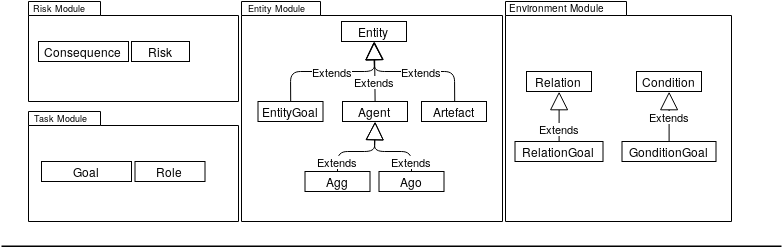
\includegraphics[width=1\linewidth]{figure/Module.png} 
	  \caption{A estrutura geral das classes do modelo}
	  \label{module}
	\end{figure} 
\end{frame}

\begin{frame}
	\frametitle{Resultados - Estrutural Conceitual - Módulos}
 	\begin{equation} 
		M_{Entity} = \{ Entity, Agent, Artefact, EntityGoal, Agg, Ago\}
	\end{equation}\label{modent}

	\begin{equation} \label{defineentity} 
		( Agent \cup Artefact ) \subset Entity
	\end{equation}

	\begin{equation} \label{agentsartefactvoid}
    	Agent \cap Artefact = \emptyset
	\end{equation}

	\begin{equation}
    	M_{Task} = \{ Goal, GoalPreRequisite, Role \}
	\end{equation}

	\begin{equation}
	    M_{Environment} = \{ Relation, ReationGoal, Condition, ConditionGoal \}
	\end{equation}

\end{frame}

\begin{frame}
	\frametitle{Resultados - Estrutural Conceitual - Predicados}
	\begin{equation}
		thereIsRelation(r_l,e_i,e_k) | r_l \in Relation \wedge  e_i, e_k \in Entity
	\end{equation}
	\begin{equation}	
		adoptsRole(ag_n,\rho_m) | ag_n \in Agent \wedge \rho_m \in Role 	
	\end{equation}
	\begin{equation}	
		hasObligation(\rho_m,g_j) | \rho_m \in Role, g_j \in Goal 
	\end{equation}		
	\begin{equation}	
		hasPermission(\rho_m, g_j) | \rho_m \in Role, g_j \in Goal
	\end{equation}
	\begin{equation}		
		isReached(g_k) | g_k \in Goal 
	\end{equation}
\end{frame}
\begin{frame}
	\frametitle{Resultados - Estrutural Conceitual - Predicados}
	\begin{equation}			
		stopIn(g_n, ag_m) | g_n \in Goal, ag_m \in Agent
	\end{equation}
	\begin{equation}			
		nextGoal(g_i,g_j) |g_i, g_j \in Goal
	\end{equation}
	\begin{equation}				
		hasCondition(g_i,cg_n) | g_i \in Goal, cg_n \subset GoalCondition
	\end{equation}
	\begin{equation}				
		hasEntity(g_i,eg_m) | g_i \in Goal, eg_m \subset EntityGoal 
	\end{equation}
	
	\begin{equation}				
		hasRelation(g_i,rg_m) | g_i \in Goal \wedge rg_m \subset RelationGoal 
	\end{equation}
\end{frame}
\begin{frame}
	\frametitle{Resultados - Estrutural Conceitual - Predicados}
	\begin{eqnarray}
	    violationEntity(ag_i,g_j,e_k) |   ag_i \in Agent \wedge g_j \in Goal \wedge \\ \nonumber 
		e_k \in Entity  
	\end{eqnarray}
	\begin{eqnarray}
	    violationRelation(ag_i,g_j,r_k) | ag_i \in Agent \wedge g_k \in Goal \wedge \\ \nonumber 
		r_k \in relation 
	\end{eqnarray}
	\begin{eqnarray}
	    violationCondition(ag_i,g_j,c_k) | ag_i \in Agent \wedge g_k \in Goal \wedge \\ \nonumber 
		c_k \in Condition 
	\end{eqnarray}
	\begin{eqnarray}
	    hasRisk(X, risk_j, cs_k) | risk_k \in Risk \wedge cs_k \in Consequence  \\ \nonumber 
	 	\wedge (X = c_k \vee X = r_k)
	\end{eqnarray}
\end{frame}
\begin{frame}
	\frametitle{Resultados - Estrutural Conceitual - Predicados}
	\begin{eqnarray}				
		isPresent(X) | X = cg_n \vee X = c_k \vee X = rg_k \vee X = r_k  \\ \nonumber
		\vee X = eg_k \vee X = e_k
	\end{eqnarray}
	\begin{equation}				
		tryReach(ag_i,g_j) | ag_i \in Agent \wedge g_j \in Goal 	
	\end{equation}
	\begin{equation}
	    possibilityHappensBadEvent(r_l) | r_l \in Relation
	\end{equation}
	\begin{equation}
	    affectsOtherRelations(r_k,r_n) | \{ r_k, r_n\} \subset Relation
	\end{equation}
	\begin{equation}
	    lastGoal(g_i,\rho_m) | g_i \in Goal, \rho_m \in Role
	\end{equation}
	\begin{equation}
		ableTryReach(ag_i,g_j) | ag_i \in Agent, g_j \in Goal,
	\end{equation}		
\end{frame}
\begin{frame}
	\frametitle{Resultados - Estrutural Conceitual - UML}
	\begin{figure}[H]
	  \centering
	  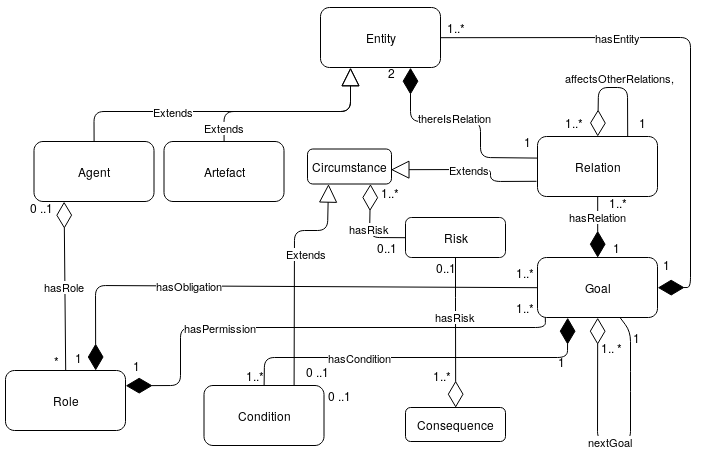
\includegraphics[width=1\linewidth]{figure/Class.png} 
	  \caption{Diagrama de classes do Modelo }
	  \label{classdiagrama}
	\end{figure}
\end{frame}
\begin{frame}
	\frametitle{Resultados - Regras}
	\begin{eqnarray}\label{reldeonticrole}
		hasObligation(\rho_m,g_j) \to hasPermission(\rho_m,g_j), \nonumber \\
	    \rho_m \in Role \wedge g_j \in Goal
	\end{eqnarray}
	\begin{eqnarray}\label{violationcondition}\nonumber
		hasCondition(g_i,cg_n) \wedge \neg isPresent(c_k) \wedge (c_k \in cg_n) \\
		\wedge tryReach(ag_m,g_i) \to \nonumber \\  
		violationCondition(ag_m,g_i,c_k) \nonumber \\  
	    g_i \in Goal, cg_n \subset ConditionGoal, c_k \in Condition, ag_m \in Agent
	\end{eqnarray}
\end{frame}
\begin{frame}
	\frametitle{Resultados - Regras}
	\begin{eqnarray}\label{violationrelation}\nonumber
		hasRelation(g_i,rg_n)\wedge \neg isPresent(r_k) \wedge (r_k \in rg_n) \\ \nonumber
		\wedge tryReach(ag_m,g_i) \to \nonumber \\
		violationRelation(ag_m,g_i,r_k) \nonumber \\  
	    g_i \in Goal, rg_n \subset RelationGoal, r_k \in Relation, ag_m \in Agent
	\end{eqnarray}
	\begin{eqnarray}\label{violationentity}\nonumber
		hasEntity(g_i,eg_n) \wedge \neg isPresent(e_k) 	\wedge (e_k \in eg_n) \\
		\wedge tryReach(ag_m,g_i) \to \nonumber \\ 
	    violationEntity(ag_m,g_i,e_k)  \nonumber \\  
	    g_i \in Goal, eg_n \subset EntityGoal, e_k \in Entity, ag_m \in Agent
	\end{eqnarray}
\end{frame}
\begin{frame}
	\frametitle{Resultados - Regras}
	\begin{eqnarray}\label{consviolationcondition}\nonumber
		violationCondition(ag_m,g_i,c_k)  \wedge  \nonumber \\ 
		hasRisk(c_k,risk_j,cs_m) \to \nonumber \\ 
		consequenceOfBadEvent(g_i,ag_m,risk_j,cs_m) \nonumber \\ 
	    ag_m \in Agent, g_i \in Goal, c_k \in Condition, \nonumber \\ 
	    risk_k \in Risk, cs_m \in Consequence \nonumber \\
	\end{eqnarray}
	\begin{eqnarray}\label{consviolationrelation}\nonumber
		violationRelation(ag_m,g_i,r_k) \nonumber \\
		\wedge hasRisk(r_k,risk_j,cs_m) \to \\ 
		consequenceOfBadEvent(g_i,ag_m,risk_j,cs_m) \nonumber \\ 
	    ag_m \in Agent, g_i \in Goal, r_k \in Relation, \nonumber \\
	    risk_k \in Risk, cs_m \in Consequence 
	\end{eqnarray}
\end{frame}
\begin{frame}
	\frametitle{Resultados - Regras}
	\begin{eqnarray}\label{violationentityaffect}
		violationRelation(ag_m,g_i,r_k) \wedge affectsOtherRelations(r_k,r_n) \nonumber \\
	    \to possibilityHappensBadEvent(r_n)  \nonumber \\
	    ag_m \in Agent, g_i \in Goal, r_k,r_n \in Relation, 
	\end{eqnarray}	
\end{frame}
\begin{frame}
	\frametitle{Resultados - Regras}
	\begin{eqnarray}\label{paybutiamnotguilty}
		possibilityHappensBadEvent(r_k) \wedge  happensBadEvent(r_k) \wedge \nonumber \\
		hasRelation(g_i,rg_n) \wedge \nonumber \\
		(r_k \in rg_n) \nonumber \\ 
		\wedge hasRisk(r_k,risk_j,cs_m) \wedge tryReach(ag_m,g_i) \nonumber \\ 
		\to consequenceOfBadEvent(g_i,ag_m,risk_j,cs_m) \nonumber \\ 
	    r_k \in Relation, g_i \in Goal, rg_n \subset RelationGoal, \nonumber \\
	     risk_k \in Risk, cs_m \in Consequence
	\end{eqnarray}
\end{frame}
\begin{frame}
	\frametitle{Resultados - Regras}
	\begin{eqnarray}\label{consvioent}
		violationEntity(ag_m,g_i,e_k) \to stopIn(g_i) \nonumber \\  
	    ag_m \in Agent, g_i \in Goal, e_k \in Entity \\ \nonumber
	\end{eqnarray}
	\begin{eqnarray}\label{badcons}
		consequenceOfBadEvent(g_k,ag_m,risk_j,cs_m) \to stopIn(g_k) \nonumber \\ 
	    g_k \in Goal, risk_j \in Risk, cs_m \in Consequence
	\end{eqnarray}
	\begin{eqnarray}\label{wenStop}
		\neg stopIn(g_k,agg_n) \wedge (ago_n \subset agg_n) \to isReached(g_k) \nonumber \\ 
	    g_k \in Goal, agg_n \in Agg, ago_n \in Ago 
	\end{eqnarray}
\end{frame}
\begin{frame}
	\frametitle{Resultados - Regras}
	\begin{eqnarray}\label{rolenextgoal}
		adoptsRole(ag_n,\rho_m) \wedge hasPermission(\rho_m,g_j) \wedge nextGoal(g_i,g_j) \nonumber \\
		\wedge isReached(g_i) \nonumber \\
		\to ableTryReach(ag_i,g_j) \nonumber \\
	    ag_i, ag_n \in Agent, \rho_m \in Role, g_j \in Goal, g_i \in Goal
	\end{eqnarray}
	\begin{eqnarray}\label{rolelastgoal}
		adoptsRole(ag_n,\rho_m) \wedge hasPermission(\rho_m,g_i) \wedge \nonumber \\
		lastGoal(g_i,\rho_m) \wedge isReached(g_i) \nonumber \\
		\to stopIn(g_i) \nonumber \\
	    ag_n \in Agent, \rho_m \in Role, g_i \in Goal
	\end{eqnarray}
\end{frame}
\begin{frame}
	\frametitle{Resultados - Tipos de Predicados}
	\begin{itemize}
		\item Fechados: $thereIsRelation(r_l,e_i,e_k)$, $adoptsRole(ag_n,\rho_m)$, $hasObligation(\rho_m,g_j)$,
		$hasPermission(\rho_m, g_j)$, $isReached(g_k)$, $stopIn(g_n, ag_m)$, $nextGoal(g_i,g_j)$, $hasCondition(g_i,cg_n)$,
		$hasEntity(g_i,eg_m)$, $hasRelation(g_i,rg_m)$, $violationCondition(ag_i,g_j,c_k) $, $ violationRelation(ag_i,g_j,r_k) $,
		$ violationEntity(ag_i,g_j,e_k) $,  $ hasRisk(X, risk_j, cs_k) $, $possibilityHappensBadEvent(r_l)$, $ableTryReach(ag_i,g_j)$ 
		$affectsOtherRelations(r_k,r_n)$, $consequenceOfBadEvenet(g_k, ag_i,risk_k,cs_m)$  e $lastGoal(g_i,\rho_m)$.
		\item Abertos: $isPresent(X)$,$tryReach(ag_i,g_j)$ e $happensBadEvent(r_m)$.
	\end{itemize}
\end{frame}
\begin{frame}
	\frametitle{Resultados - Caso de Estudo}
	\begin{itemize}
		\item O estudo de caso desta pesquisa consiste em sete profissionais de linha viva.
		\item Um supervisor e seis executores.
		\item Céu ensolarado e umidade relativa do ar menor que 70 porcento.
		\item EPI's necessários: capacete, óculos de sol, roupa isolante e antichamas, luvas isolantes e botas isolantes.
		\item  bastão garra de diâmetro 64 x 3600 mm, sela de diâmetro 65, colar, corda de fibra sintética, carretilha, chave com catraca, bastão universal, soquete adequado, locador de pino e bastão com soquete multiangular
		\item O método selecionado para esse tipo de manutenção é a distância.
	\end{itemize}
\end{frame}
\begin{frame}
	\frametitle{Resultados - Raciocínio 1}
	\begin{enumerate}
		\item $adoptsRole(agente4,executor2)$ 
		\item $hasObligation(executor2,g1)$
		\item $hasRelation(g1,rg1)$ 
		\item $relPanoCorda \in rg1$
		\item $ x = agente4 $
		\item $tryReach(agente4,g1)$
		\item $affectsOtherRelations(relPanoGlicerina,relBastaoGarraCondutor)$
		\item $affectsOtherRelations(relPanoGlicerina,relCordaEstropo)$  
		\item $affectsOtherRelations(relPanoGlicerina,relChaveCatracaParafuso)$
		\item $affectsOtherRelations(relPanoGlicerina,relParafusoConector)$ 
		\item $affectsOtherRelations(relPanoGlicerina,relSoqueteParafuso)$ 
		\item $affectsOtherRelations(relPanoGlicerina,relAgente4Corda)$ 
		\item $affectsOtherRelations(relPanoGlicerina,relEstropoCorda)$	
	\end{enumerate}
\end{frame}
\begin{frame}
	\frametitle{Resultados - Raciocínio 1}
	\begin{eqnarray}\nonumber
		hasRelation(g1,rg1)\wedge \neg isPresent(relPanoGlicerina)  \nonumber \\ 
		\wedge (relPanoGlicerina\in rg_1) \wedge tryReach(agente4,g1) \nonumber \\ 
		\to \nonumber \\ 
		violationRelation(agente4,g1,relPanoGlicerina) \nonumber \\	
	\end{eqnarray}
	\begin{eqnarray}\nonumber
		violationRelation(agente4,g1,relPanoGlicerina)  \nonumber \\ 
		\wedge affectsOtherRelations(relPanoGlicerina,relBastaoGarraCondutor)   \nonumber \\ 
		\to \nonumber \\  
		possibilityHappensBadEvent(relBastaoGarraCondutor) 
	\end{eqnarray}
\end{frame}
\begin{frame}
	\frametitle{Resultados - Raciocínio 2}
	\begin{enumerate}
		\item $adoptsRole(agente2,executor1)$ 
		\item $adoptsRole(agente3,executor1)$	 	
		\item $adoptsRole(agente4,executor2)$	 
		\item $hasObligation(executor1,g1)$
		\item $hasObligation(executor2,g1)$
		\item $tryReach(agente2,g1)$ 
		\item $tryReach(agente3,g1)$	 	
		\item $tryReach(agente4,g1)$	
		\item $hasEntity(g1,eg1)$		
		\item $pano \in eg1$
		\item $\neg isPresent(pano)$
	\end{enumerate}
\end{frame}
\begin{frame}
	\frametitle{Resultados - Raciocínio 2}
	\begin{eqnarray}\nonumber
		hasEntity(g1,eg1) \nonumber \\ 
		\wedge \neg isPresent(pano) 	\nonumber \\ 
		\wedge (pano \in eg1) \wedge tryReach(agente2,g1) \to \nonumber \\ 
		violationEntity(agent2,g1,pano) \nonumber \\
	\end{eqnarray}

	\begin{eqnarray}\nonumber
		hasEntity(g1,eg1) \nonumber \\ 
		\wedge \neg isPresent(pano) 	\nonumber \\ 
		\wedge (pano \in eg1) \wedge tryReach(agente3,g1) \to \nonumber \\ 
		violationEntity(agente3,g1,pano) \nonumber \\
	\end{eqnarray}

\end{frame}
\begin{frame}
	\frametitle{Resultados - Raciocínio 2}
	\begin{eqnarray}\nonumber
		hasEntity(g1,eg1) \nonumber \\ 
		\wedge \neg isPresent(pano) 	\nonumber \\ 
		\wedge (pano \in eg1) \wedge tryReach(agente4,g1) \to \nonumber \\ 
		violationEntity(agente4,g1,pano) \nonumber \\
	\end{eqnarray}

	\begin{eqnarray}
		violationEntity(agente4,g1,pano) \to stopIn(g1)
	\end{eqnarray}
\end{frame}

\begin{frame}
	\frametitle{Resultados - Raciocínio 3}
	\begin{enumerate}
		\item $adoptsRole(agente5,executor3)$
		\item $hasObligation(executor3,g11)$	
		\item $tryReach(agente5,g11)$ 
		\item $hasCondition(g11,cg1)$
		\item $umidade70 \in cg1$	
		\item $\neg isPresent(umidade70)$
		\item $hasRisk(umidade70,eletrocutado,morte)$
	\end{enumerate}
\end{frame}

\begin{frame}
	\frametitle{Resultados - Raciocínio 3}
	\begin{eqnarray}
		hasCondition(g11,cg1) \nonumber \\ 
		\wedge \neg isPresent(umidade70) \nonumber \\
		\wedge umidade70 \in cg1 \nonumber \\
		\wedge tryReach(agente5,g11) \to \nonumber \\  
		violationCondition(agente5,g11,umidade70) 
	\end{eqnarray}

	\begin{eqnarray} \nonumber
		violationCondition(agente5,g11,umidade70) \nonumber \\
		\wedge hasRisk(umidade70,eletrocutado,morte) \to \nonumber \\  
		consequenceOfBadEvent(g11,agente5,eletrocutado,morte)
	\end{eqnarray}

	\begin{eqnarray}
		consequenceOfBadEvent(g11,agente5,eletrocutado,morte) \\ \nonumber \to stopIn(g11) \nonumber
	\end{eqnarray}	
\end{frame}

\begin{frame}
	\frametitle{Resultados - Raciocínio 4}
	\begin{enumerate}
		\item $adoptsRole(agente4,executor2)$
		\item $hasObligation(executor4,g15)$	
		\item $tryReach(agente4,g15)$ 
		\item $hasRelation(g15,rg15)$
		\item $relChaveCatracaParafuso \in rg15$	
		\item $\neg isPresent(relChaveCatracaParafuso)$
		\item $hasRisk(relChaveCatracaParafuso,eletrocutado,morte)$
	\end{enumerate}
\end{frame}

\begin{frame}
	\frametitle{Resultados - Raciocínio 4}
	\begin{eqnarray}
		hasRelation(g15,rg15) \wedge \neg isPresent(relChaveCatracaParafuso)  \nonumber \\ 
		\wedge (relChaveCatracaParafuso \in rg15) \nonumber \\
		\wedge tryReach(agente4,g15) \nonumber \\ 
		\to \nonumber \\ 
		violationRelation(agente4,g15,relChaveCatracaParafuso) \nonumber \\
	\end{eqnarray}
	\begin{eqnarray}\nonumber
		violationRelation(agente4,g15,relChaveCatracaParafuso) \nonumber \\ 
		 \wedge hasRisk(relChaveCatracaParafuso,eletrocutado,morte) \nonumber \\ 
		\to \nonumber \\ 
		consequenceOfBadEvent(g15,agente4,eletrocutado,morte)
	\end{eqnarray}
	\begin{eqnarray}
		consequenceOfBadEvent(g15,agente4,eletrocutado,morte) \nonumber \\ 
		\to stopIn(g15)
	\end{eqnarray}
\end{frame}

\begin{frame}
	\frametitle{Resultados - Raciocínio 5}
	\begin{enumerate}
		\item $relParafusoConector \in rg19$	
		\item $hasRelation(g19,rg19)$		
		\item $hasObligation(executor3,g19)$
		\item $hasObligation(executor4,g19)$
		\item $hasObligation(executor5,g19)$		
		\item $tryReach(agente5,g19)$
		\item $tryReach(agente6,g19)$
		\item $tryReach(agente7,g19)$									
		\item $adoptsRole(agente5,executor3)$
		\item $adoptsRole(agente6,executor4)$
		\item $adoptsRole(agente7,executor5)$
		\item $hasRisk(relParafusoConector,eletrocutado,morte)$
		\item $possibilityHappensBadEvent(relParafusoConector)$
		\item $happensBadEvent(g19,relParafusoConector)$	
	\end{enumerate}
\end{frame}

\begin{frame}
	\frametitle{Resultados - Raciocínio 5}
	\begin{eqnarray}\nonumber
	    possibilityHappensBadEvent(relParafusoConector) \nonumber \\
	    \wedge happensBadEvent(relParafusoConector) \nonumber \\ 
	    \wedge hasRelation(g19,rg19)  \nonumber \\  
	    \wedge (relParafusoConector \in rg19) \nonumber \\ 
	    \wedge hasRisk(relParafusoConector,eletrocutado,morte) \nonumber \\  
	    \wedge tryReach(agente5,g19) \nonumber \\ 
	    \to consequenceOfBadEvent(g19,agente5,eletrocutado,morte) \\ \nonumber
	\end{eqnarray}
	\begin{eqnarray}
		consequenceOfBadEvent(g19,agente5,eletrocutado,morte) \nonumber \\ 
		\to stopIn(g19)
	\end{eqnarray}
\end{frame}

\begin{frame}
	\frametitle{Resultados - Raciocínio 6}
	\begin{enumerate}
		\item $agente2 \in agg23$	
		\item $agente3 \in agg23$
		\item $agente4 \in agg23$
		\item $agente5 \in agg23$
		\item $agente7 \in agg23$								
		\item $agente2 \in ago23$	
		\item $agente3 \in ago23$
		\item $agente4 \in ago23$
		\item $agente5 \in ago23$
		\item $agente7 \in ago23$	
		\item $ago23 \subset agg23$
		\item $\neg stopIn(g23,agg23)$										
	\end{enumerate}
	\begin{eqnarray}\label{rel15}
		\neg stopIn(g23,agg23) \wedge (ago23 \subset agg23) \to isReached(g23)
	\end{eqnarray}
\end{frame}
\begin{frame}
	\frametitle{Discussão - Critérios de Comparação}
	\begin{itemize}
		\item \textbf{Agente} condiz numa representação dos estados internos que um agente pode ter
		\item O critério \textbf{SMA} condiz na presença de elementos que são necessário para especificar um \textit{Sistema Multiagente}
		\item O critério \textbf{Artefato} condiz com elementos que correspondem ao tratado na Fundamntação Teórica.
		\item \textbf{Norma} corresponde a regras que devem ser acatadas pelos agentes 
		\item \textbf{Violação} define o que corresponde o não cumprimento de uma dada regra
		\item \textbf{Sanção} implica penalidade que está sobre o agente.
		\item \textbf{Risco} consiste no evento ruim que tem um dado potencial de ocorrer sobre o agente
	\end{itemize}
\end{frame}
\begin{frame}
	\frametitle{Discussão - Critérios de Comparação}
	\begin{itemize}
		\item \textbf{P.O.A.E} significa Possibilidade de Ocorrer algo Errado.
		\item \textbf{Objetivos} implica alvos que devem ser atingidos pelos agentes 
		\item \textbf{C.A} consiste em condições ambientes que interagem com a atividade executada pelos agentes.
		\item \textbf{I.AG.AR} representa as interações entre agentes e artefatos
		\item \textbf{D.C.A} - Descrição de Cenários de Acidentes, consiste na capacidade de desenvolver raciocínios a fim de representar cenários de acidentes.
	\end{itemize}
\end{frame}
\begin{frame}
	\frametitle{Discussão - Expressividade}
	\begin{itemize}
			\item nenhuma expressividade - o engenheiro de modelagem terá de criar uma estrutura conceitual grande e complexa. 
			\item pouco expressivo - possui algumas estruturas pré-definidas que diminuem o esforço da especificação. 
			\item expressivo - o modelo permite especificar o objeto de interesse sem que o engenheiro tenha de criar muitos atributos para o domínio de interesse.
			\item muito expressivo - o modelo apresenta diversos conceitos específicos para representar o objeto em interesse
			\item altamente expressivo - o modelo especifica o objetivo de interesse muito bem fazendo com que o engenheiro de conhecimento não tenha que definir nenhum critério conceitual a mais.
	\end{itemize}
\end{frame}
\begin{frame}
	\frametitle{Discussão - Análise Comparativa - MOISE+}
	\begin{table}[H]
	    \begin{tabular}{|l|l|l|l|l|l|}
	        \textbf{Critérios} 	&	 \textbf{MOISE+}        	&	 \textbf{MODELO DESTE ESTUDO} \\ \hline
	        \textbf{Agente}    	&	 pouco expressivo       	&	 pouco expressivo             \\ \hline
	        \textbf{SMA}       	&	 altamente expressivo   	&	 expressivo                   \\ \hline
	        \textbf{Artefato}  	&	 nenhuma expressividade 	&	 expressivo                   \\ \hline
	        \textbf{Norma}     	&	 nenhuma expressividade 	&	 altamente expressivo         \\ \hline
	        \textbf{Violação}  	&	 nenhuma expressividade 	&	 altamente expressivo         \\ \hline
	        \textbf{Sanção}    	&	 nenhuma expressividade 	&	 altamente expressivo         \\ \hline
	        \textbf{Risco}     	&	 nenhuma expressividade 	&	 muito expressivo             \\ \hline
	        \textbf{P.O.A.E}   	&	 nenhuma expressividade 	&	 altamente expressivo         \\ \hline
	        \textbf{Objetivos} 	&	 muito expressivo       	&	 expressivo             \\ \hline
	        \textbf{C.A}       	&	 nenhuma expressividade 	&	 muito expressivo             \\ \hline
	        \textbf{I.AG.AR}   	&	 nenhuma expressividade 	&	 muito expressivo             \\ \hline
	        \textbf{D.C.A}     	&	 nenhuma expressividade 	&	 muito expressivo             \\ \hline
	    \end{tabular}
	\end{table}
\end{frame}

\begin{frame}
	\frametitle{Discussão - Análise Comparativa - DASTANI}
	\begin{table}[H]
	    \begin{tabular}{|l|l|l|l|l|l|}
	            \textbf{Critérios} 	&	 \textbf{DASTANI}     	&	 \textbf{MODELO DESTE ESTUDO} \\ \hline
		        \textbf{Agente}    	&	 pouco expressivo     	&	 pouco expressivo             \\ \hline
		        \textbf{SMA}       	&	 pouco expressivo     	&	 expressivo                   \\ \hline
		        \textbf{Artefato}  	&	 pouco expressivo     	&	 expressivo                   \\ \hline
		        \textbf{Norma}     	&	 altamente expressivo 	&	 altamente expressivo         \\ \hline
		        \textbf{Violação}  	&	 altamente expressivo 	&	 altamente expressivo         \\ \hline
		        \textbf{Sanção}    	&	 altamente expressivo 	&	 altamente expressivo         \\ \hline
		        \textbf{Risco}     	&	 pouco expressivo     	&	 muito expressivo             \\ \hline
		        \textbf{P.O.A.E}   	&	 pouco expressivo     	&	 altamente expressivo         \\ \hline
		        \textbf{Objetivos} 	&	 pouco expressivo     	&	 expressivo             	  \\ \hline
		        \textbf{C.A}       	&	 pouco expressivo     	&	 muito expressivo             \\ \hline
		        \textbf{I.AG.AR}   	&	 pouco expressivo     	&	 muito expressivo             \\ \hline
		        \textbf{D.C.A}     	&	 pouco expressivo     	&	 muito expressivo             \\ \hline
	    \end{tabular}
	\end{table}
\end{frame}

\begin{frame}
	\frametitle{Discussão - Análise Comparativa - NORMMAS}
	\textbf{Definição 1.} \textit{Um norma é definida por meio de uma tupla} $N = \langle \mu,\kappa,\chi,\tau,\rho \rangle$

	\begin{itemize}
	    \item $\mu \in \{obligation,prohibition\}$ representa as modalidades de norma.
	    \item $\kappa \in \{action,state\}$ representa o tipo de \textit{trigger} da condição.
	    \item $\chi$ representa o conjunto de estados em que uma norma se aplica.
	    \item $\tau$ representa a norma da condição de \textit{trigger}
	    \item $\rho$ representa a sanção aplicava pela violação do agente.
	\end{itemize}

	A definição 1 pode ser compreendida sobre o seguinte exemplo; 

	\textit{Todos os imigrantes que possuem passaporte válido, devem ser aceitos. A falha resulta na perda de 5 créditos}. 

	Dentro da definição 1, o exemplo fica;
	\begin{eqnarray}
	    \langle obligation,action,valid(Passport),accept(Passport),loss(5)\rangle
	\end{eqnarray}

	\begin{eqnarray}
	    \langle obligation,action,valid(Passport),accept(Passport),loss(5)\rangle
	\end{eqnarray}
\end{frame}

\begin{frame}
	\frametitle{Discussão - Análise Comparativa - NORMMAS}
\textbf{Definição 2.} \textit{Um Registro de Ação é definido por meio de uma tupla} $R = \langle \gamma,\alpha,\beta \rangle$
	\begin{itemize}
	    \item $\gamma$ representa o agente executando uma ação;
	    \item $\alpha$ representa a ação sendo executada pelo agente $\gamma$
	    \item $\beta$ representa os estados internos do agente $\gamma$ no momento da execução.
	\end{itemize}

	Para demonstrar como se dá o uso dessa definição pode-se considerar a seguinte sentença;

	\textit{O oficial John aprovou passaport 3225. O passaporte 3225 é definido como validado.}

	Nessa sentença, $John$ é o agente dado por $\gamma$, o ato de aprovar o passaporte é o $\gamma$ que pode ser definido pelo predicado por $approve(3225)$ e o estado de ser validado por ser dado pelo predicado $valid(3225)$.  

	Usando a \textbf{Definição 2}, isso poder ser especificado da seguinte maneira; 
	\begin{eqnarray}
	    \langle John, approve(3225), valid(3225)\rangle
	\end{eqnarray}
\end{frame}


\begin{frame}
	\frametitle{Discussão - Análise Comparativa - NORMMAS}
	\begin{table}[H]
	    \begin{tabular}{|l|l|l|l|l|l|}
	        \textbf{Critérios} 	&	 \textbf{NORMMAS}     	&	 \textbf{MODELO DESTE ESTUDO} \\ \hline
	        \textbf{Agente}    	&	 pouco expressivo     	&	 pouco expressivo             \\ \hline
	        \textbf{SMA}       	&	 pouco expressivo     	&	 expressivo                   \\ \hline
	        \textbf{Artefato}  	&	 pouco expressivo     	&	 expressivo                   \\ \hline
	        \textbf{Norma}     	&	 altamente expressivo 	&	 altamente expressivo         \\ \hline
	        \textbf{Violação}  	&	 altamente expressivo 	&	 altamente expressivo         \\ \hline
	        \textbf{Sanção}    	&	 altamente expressivo 	&	 altamente expressivo         \\ \hline
	        \textbf{Risco}     	&	 pouco expressivo     	&	 muito expressivo             \\ \hline
	        \textbf{P.O.A.E}   	&	 pouco expressivo     	&	 altamente expressivo         \\ \hline
	        \textbf{Objetivos} 	&	 pouco expressivo     	&	 expressivo             	  \\ \hline
	        \textbf{C.A}       	&	 pouco expressivo     	&	 muito expressivo             \\ \hline
	        \textbf{I.AG.AR}   	&	 pouco expressivo     	&	 muito expressivo             \\ \hline
	        \textbf{D.C.A}     	&	 pouco expressivo     	&	 muito expressivo             \\ \hline
	    \end{tabular}
	\end{table}
\end{frame}

\begin{frame}
	\frametitle{Discussão - Análise Comparativa - V3S}
	\begin{itemize}
		\item V3S é um modelo com a finalidade de gerar ambientes para desenvolver treinamentos complexos em ambiente de realidade virtual visando atividades de risco e de emergência.
		\item \textit{Domain Model}, \textit{Activity Model} e \textit{Risk Model}
	\end{itemize}
	\begin{figure}[H]
	  \centering
	  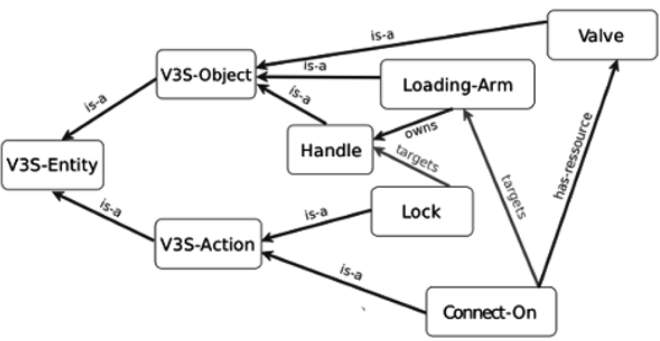
\includegraphics[width=0.4\linewidth]{figure/ontologyv3.png} 
	  \caption{Ontologia que descreve \textit{Domain Model} no model V3S \cite{v3sframework}}
	  \label{domainmodel}
	\end{figure}
\end{frame}

\begin{frame}
	\frametitle{Discussão - Análise Comparativa - V3S}
	\begin{itemize}
		\item Activity Mode; Possui uma linguagem para descrever atividades denominada por; álgebra de Allen's
		\item \textit{ACTIVITY-DL} incorpora os conceitos de BCTUs e BATUs
		\item Risck Model: Faz uso do projeto MELISSA (combinação entre análise quantitativa com análise qualitativa).
		\item MELISSA representa os cenário de acidente por meio do gráfico \textit{Bowtie}
		\item \textit{V3S} trabalha com o conceito de personagens virtuais que são representados usando \textit{framework} MASVERP.
		\item \textit{HERA}, por intermédio de regras baseadas em modelos pedagógicos, fornece o respaldo ao instrutor.
	\end{itemize}
\end{frame}

\begin{frame}
	\frametitle{Discussão - Análise Comparativa - V3S}
	\begin{table}[H]
	    \begin{tabular}{|l|l|l|l|l|l|}
        \textbf{Critérios} 	&	 \textbf{V3S}         	&	 \textbf{MODELO DESTE ESTUDO} \\ \hline
        \textbf{Agente}    	&	 muito expressivo     	&	 pouco expressivo             \\ \hline
        \textbf{SMA}       	&	 expressivo           	&	 expressivo                   \\ \hline
        \textbf{Artefato}  	&	 expressivo           	&	 expressivo                   \\ \hline
        \textbf{Norma}     	&	 pouco expressivo     	&	 altamente expressivo         \\ \hline
        \textbf{Violação}  	&	 pouco expressivo     	&	 altamente expressivo         \\ \hline
        \textbf{Sanção}    	&	 pouco expressivo     	&	 altamente expressivo         \\ \hline
        \textbf{Risco}     	&	 altamente expressivo 	&	 muito expressivo             \\ \hline
        \textbf{P.O.A.E}   	&	 pouco expressivo     	&	 altamente expressivo         \\ \hline
        \textbf{Objetivos} 	&	 muito expressivo       &	 expressivo             	  \\ \hline
        \textbf{C.A}       	&	 pouco expressivo     	&	 muito expressivo             \\ \hline
        \textbf{I.AG.AR}   	&	 pouco expressivo     	&	 muito expressivo             \\ \hline
        \textbf{D.C.A}     	&	 altamente expressivo 	&	 muito expressivo             \\ \hline
	    \end{tabular}
	\end{table}	
\end{frame}

\begin{frame}
	\frametitle{Discussão - Consistência dos Resultados - Caso de Estudo}
	\begin{itemize}
		\item  O caso em análise cumpre com os interesses da pesquisa pois apresenta um cenário onde profissionais usam ferramentas para trabalhar de forma colaborativa a fim de atingir um determinado objetivo
		\item Os profissionais são expostos a um dado risco e podem sofrer acidentes que advêm tanto de responsabilidade própria bem como responsabilidade do outro.
		\item A compreensão da atividade propriamente dita não foi uma tarefa fácil e exigiu grande esforço do autor
		\item O caso de estudo em análise é um cenário que é totalmente possível de ser factual, contudo existe diversas outras possibilidades de organizar a mesma manutenção.
	\end{itemize}
\end{frame}


\begin{frame}
	\frametitle{Discussão - Consistência dos Resultados - Caso de Estudo}
	\begin{itemize}
		\item A primeira fase consistiu em descrever a manutenção em termos de objetivos que as vezes são organizados em série e as vezes em paralelo
		\item Um ponto  complicado de se verificar nesse estudo se deve ao fato de que os profissionais não precisam executar os objetivos na estrutura em que o modelo foi apresentado.
		\item Há um número finito e relativamente pequeno sobre como esses objetivos podem ser organizados e isso ameniza a falta de previsibilidade de como a manutenção será realizada.
		\item Solução para essa questão; 1 - Engenheiro de Manutenção organiza os objetivos de todas formas possíveis, 2 - Definir todas as relações possíveis que o predicado $nextGoal(g_i,g_j)$ permite em uma única estrutura.
	\end{itemize}
\end{frame}


\begin{frame}
	\frametitle{Discussão - Consistência dos Resultados - Conceitos}
	\begin{itemize}
		\item "Papel" foi adequado para especificar a função dos agentes.
		\item "Artefact" foi adequado para especificar todas as ferramentas e equipamentos.
		\item Sem "Condition" seria impossível determinar como o meio interfere na manutenção.
		\item A modelagem trabalhou apenas sobre o risco de ser eletrocutado com uma única consequência que é de morte. Apesar de na prática não ser a única, é a principal e gera maior preocupação. Além disso, essa questão não corrobora negativamente paras demonstrações.
		\item O mapeamento de todas realações que podem ser concebidas entre as entidades (sempre duas) foi interessante porque permitiu descrever a manutençao com muita riqueza de detalhes. Contudo o processo também foi custoso, pois exige muito tempo e esforço em mapear cada relação.  
	\end{itemize}
\end{frame}

\begin{frame}
	\frametitle{Discussão - Consistência dos Resultados - Conceitos}
	\begin{itemize}
		\item $affectsOtherRelations(r_k,r_n)$ - abstraiu muito as relações de causalidade, contudo permitiu conceber um modelo que considera esse tipo de situação.
		\item Esse estudo mostrou que permitir a especificação do predicado $hasEntity(g_i,eg_j)$ e do predicado $hasRelation(g_i,rg_j)$ pode levar o modelador a contradições;
		\item Ex; um objetivo $g_1$ é constituído por $e_1,e_2,e_3$ e é formado pelas relações $thereIsRelation(r_{12},e_1,e_2)$ e $thereIsRelation(r_{23},e_2,e_3)$, $rg_1 = \{ r_{12},r_{23} \}$ e $ eg_1 = \{ e_1, e_2 \} $, $ hasEntity(g_1,eg_1) $ e $ hasRelation(g_1, rg_1) $ $rg_{23}$. 
		\item Esse problema pode ser resolvido por desconsiderar o predicado $hasEntity(g_n,eg_m)$ tendo em vista que um simples raciocínio usando $hasRelation(g_n,rg_m)$, $r_k \in rg_m$ e $thereIsRelation(r_k, e_a,e_b)$.
	\end{itemize}
\end{frame}

\begin{frame}
	\frametitle{Discussão - Consistência dos Resultados - Raciocínios}
	\begin{itemize}
		\item O Raciocínio 1 foi realmente apropriado para descrever como se dá na prática quando alguém esquece de executar uma relação. Por conta disso o autor dessa dissertação entendeu que esse raciocínio é um fator relevante para cumprir em partes com os objetivos 2 (pois considerar o erro do agente) em partes com objetivo  3 e 5 (pois é essencial para compreender quais são as relações com possibilidade de acidentes). 
		\item O Raciocínio 2 corresponde a realidade onde a ausência de um pano realmente impede o prosseguimento da manutenção. Contudo, cenário que não foi explorado por esse modelo consiste na adaptação de objetos como ferramentas. Apesar disso, o raciocínio foi eficaz em representar o cenário realistico e conservador. Portanto esse raciocínio cumpre com os objetivos 2 (pois considera norma, violação e sanção) e cumpre, em partes, com objetivo 4.
	\end{itemize}
\end{frame}


\begin{frame}
	\frametitle{Discussão - Consistência dos Resultados - Raciocínios}
	\begin{itemize} 
		\item O Racicínio 3 exibe um cenário de mundo real, uma vez que não respeito as condições ambientais pode acarregar consequências trágicas. Contudo, não aborda a possibilidade do profissional cometer esse tipo de violação e não sofrer as penalidades. Uma maneira de corrigir isso consiste considerar o uso do predicado $possibilityHappensBadEvent(r_l)$. Por outro lado, dessa maneira o modelo retrata sempre o pior cenário. Por conta disso, esse raciocínio cumpre com objetivo 4;
		\item O raciocínio 4 retrata um cenário factual do profissional manipular a ferramenta de forma inaproprieada. Porém, assim como no raciocínio 3, não considera a possibilidade do agente cometer algum equívoco sem se ferir gravemente. Ainda sim, retrata um cenário factível e conservador. Tendo em vista isso, esse raciocínio cumpre com objetivo 2 e em partes com objetivo 4. 
	\end{itemize}
\end{frame}

\begin{frame}
	\frametitle{Discussão - Consistência dos Resultados - Raciocínios}
	\begin{itemize} 
		\item O raciocínio 5 descreve um cenário onde, por um erro ocorrido no raciocínio 1, outros profissionais sofrem consequências negativas. Esse raciocínio corresponde a realidade dos fatos para essa especificação. Em conjunto com o raciocínio 1, cumpre com os objetivos 3 e 5.
		\item Todos os raciocínios consideram elementos de uma SMA, cumprindo con o objetivo 1.  
	\end{itemize}
\end{frame}


\begin{frame}
	\frametitle{Conclusão}
	\begin{itemize} 
		\item Foi possível chegar em um modelo que está de acordo com os objetivos dessa pesquisa e que aborda essa problemática de forma diferente dos modelos atuais.
		\item O cenário foi especificado com sucesso e todos os raciocínios representaram cenários reais. Contudo não foram suficientes para representar todos os cenários possíveis.
		\item Criar estruturas dentro dessa representação que possam tratar desses outros cenários. 
		\item Trabalhar com a idéia de probabilidade em vez de possibilidade.   
	\end{itemize}
\end{frame}


\end{document} 	
